% TODO(team): Maintain the checkpoint text and its supporting citations.
\documentclass[letterpaper,twocolumn,10pt]{article}
\usepackage{usenix-2020-09}
\usepackage{amsmath}
\usepackage{tikz}
\usetikzlibrary{arrows.meta,positioning}
\hypersetup{hidelinks,pdftitle={COMPSCI 512 Project Checkpoint: Cooperative Video Storage and Streaming},pdfauthor={Haoyu Wang, Yuquan Hu, Tian Xia}}

\begin{document}
\date{}
\title{\Large\bf Cooperative Video Storage and Streaming\\COMPSCI 512 Project Checkpoint}
\author{{\rm Haoyu Wang}\\hw418@duke.edu
\and {\rm Yuquan Hu}\\yh511@duke.edu
\and {\rm Tian Xia}\\tx55@duke.edu}
\maketitle

\section{Motivation and Research Question}
A group of machines can pool limited storage to host a video library larger than any individual machine can hold. However, heterogeneous upload capacity, temporary disconnections, and concentrated demand can make stored videos unavailable at playback deadlines. Our proposal combines distributed segment storage, replicated metadata, and direct peer-to-peer delivery. This checkpoint develops the design and evaluation plan; implementation progress and experimental results have not yet been verified.

Our central hypothesis is that \emph{jointly considering segment urgency, popularity, and peer availability reduces rebuffering relative to fixed replication and independent request scheduling, under identical storage and upload budgets}. A secondary question is whether erasure coding for cold segments saves enough space to justify decoding and repair costs. These are hypotheses, not established improvements. The intended contribution is an implementation and controlled study of these interactions in a small cooperative deployment, rather than a new consensus or coding algorithm.

\section{Background and Related Work}
\paragraph{Storage efficiency and recovery.}
Replication permits a direct read from any surviving copy, but consumes one
full segment per replica. Erasure coding stores $k$ data and $m$ parity
fragments and reconstructs a segment from any $k$ distinct fragments, at
storage overhead $(k+m)/k$. HACFS~\cite{xia2015tale} adapts between a fast
and a compact erasure code to trade recovery cost against storage overhead.
It does not implement our proposed hot-replica/cold-code policy. We borrow
this tradeoff and investigate its effect on video deadlines and peer upload
budgets.

The Google File System~\cite{ghemawat2003gfs} separates a centralized
metadata service from direct transfers between clients and chunkservers,
and uses checksums, replication, and automatic repair to tolerate component
failures. This separation motivates our decision to keep video bytes outside
the metadata log. Total Recall~\cite{bhagwan2004totalrecall} estimates peer
availability from observed behavior and automatically adjusts redundancy and
repair policies. Our placement controller similarly considers peer
availability, but additionally accounts for segment popularity, playback
deadlines, and explicit storage and upload budgets.

\paragraph{Streaming and caching.}
Hsu and Hefeeda~\cite{hsu2010quality} formulate quality-aware segment
scheduling in mesh-based streaming, establish its computational difficulty,
and develop an approximation algorithm. Our initial client uses a lightweight
deadline heuristic, with no optimality guarantee, and evaluates it together
with storage placement. CoolStreaming/DONet~\cite{zhang2005coolstreaming}
demonstrates a data-driven overlay in which peers exchange availability
information and retrieve missing video segments from multiple partners. This
supports our use of direct multi-peer delivery without requiring a fixed
distribution tree.

A large-scale study of the PPLive P2P-VoD
system~\cite{huang2008p2pvod} identifies segmentation, content replication,
content discovery, peer scheduling, and playback fluency as central design
and evaluation concerns. These mechanisms closely match our proposed peer
stores and deadline-aware client. SPACE~\cite{aguilar2023space} studies edge
prefetching and caching for adaptive streaming, including popularity-based
caching. Our setting differs because peers hold the durable library:
eviction must preserve recoverability, and an origin server cannot always
supply missing segments. Thus, popularity alone is insufficient for
placement.

\paragraph{Coordination and redundant work.}
Raft~\cite{ongaro2014raft} supplies consistency for metadata and task records;
it does not protect video bytes outside the log. ZooKeeper~\cite{hunt2010zookeeper}
shows how a replicated coordination service can expose a small, consistent
interface from which applications construct higher-level mechanisms. Our
metadata service follows the same separation of concerns, but directly stores
video manifests, acknowledged locations, representation versions, and repair
task transitions.

MapReduce~\cite{dean2004mapreduce} motivates periodically aggregating peer
observations, but we plan a small aggregation worker rather than a full batch
framework. Dean and Barroso~\cite{dean2013tail} explain how rare slow
responses can dominate the latency of distributed operations and describe
redundant requests as one tail-tolerance technique. Primorac et
al.~\cite{primorac2021hedge} further show that redundant requests can worsen
congestion and need not improve latency over good load balancing.
Accordingly, our client will bound duplicate transfers and measure their
cost. Our question concerns the interaction of established mechanisms, not
an assertion that their combination is unprecedented.

\section{High-Level Design}
\subsection{Components, Data Model, and Assumptions}
Figure~\ref{fig:architecture} separates metadata coordination from video delivery. We target trusted peers on a reachable LAN or VPN, with crash/restart failures and network partitions. Byzantine behavior, NAT traversal, transcoding, and adaptive bitrate selection are outside the initial scope. A fixed video representation and configurable segment duration isolate storage and scheduling effects.

\begin{figure}[t]
\centering
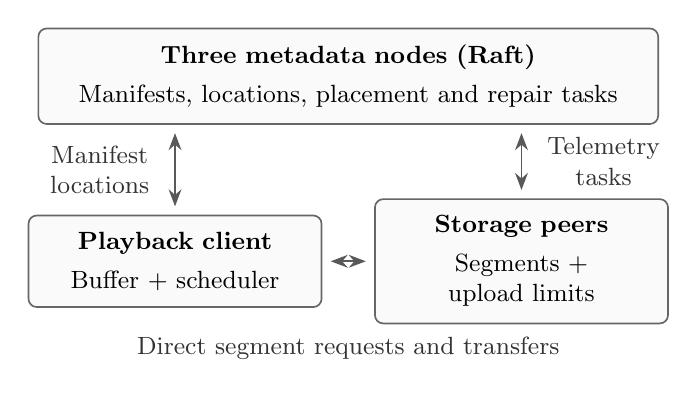
\begin{tikzpicture}[
 font=\small,
 >=Stealth,
 box/.style={draw=black!60,fill=black!2,rounded corners=3pt,
   line width=0.6pt,align=center,inner sep=6pt,minimum height=1.05cm},
 flow/.style={<->,draw=black!65,line width=0.7pt,
   shorten <=3pt,shorten >=3pt},
 flowlabel/.style={align=center,inner sep=2pt,text=black!80}
]
\node[box,text width=7.45cm] (meta) at (0,0)
 {\textbf{Three metadata nodes (Raft)}\\[3pt]
  Manifests, locations, placement and repair tasks};
\node[box,text width=3.3cm] (client) at (-2.2,-2.35)
 {\textbf{Playback client}\\[3pt]Buffer + scheduler};
\node[box,text width=3.3cm] (peers) at (2.2,-2.35)
 {\textbf{Storage peers}\\[3pt]Segments + upload limits};
\draw[flow] (client.north) --
 node[flowlabel,midway,left=7pt]{Manifest\\locations}
 (client.north |- meta.south);
\draw[flow] (peers.north) --
 node[flowlabel,midway,right=7pt]{Telemetry\\tasks}
 (peers.north |- meta.south);
\draw[flow] (client.east) -- (peers.west);
\node[flowlabel] at (0,-3.45)
 {Direct segment requests and transfers};
\end{tikzpicture}
\caption{Proposed architecture. Video bytes bypass Raft.}
\label{fig:architecture}
\end{figure}

An immutable manifest records segment order, duration, byte length, and SHA-256 hash; coded segments also record code parameters and fragment hashes. Mutable metadata maps object IDs to acknowledged locations and representation versions. A peer writes a temporary object, verifies its hash, durably installs it, and acknowledges completion before its location is advertised. Ingestion publishes a video only after every segment meets the initial redundancy target. Hashes detect accidental corruption; they do not authenticate an untrusted publisher.

We plan peer and controller services in Go, using a maintained Raft library, HTTP segment transfers, and a client feeding ordered segments to a local player. Three controllers will replicate manifests, location updates, and task transitions. High-rate telemetry remains soft state; a new leader refreshes it before scheduling. Cached manifests and reachable peers may sustain playback during a controller outage, while metadata changes require a quorum.

\subsection{Placement, Repair, and Resource Limits}
The first implementation will keep two replicas of each segment on distinct peers. A periodic scheduler will rank optional third copies by recent request count, with extra weight for the startup prefix. It will choose destinations using free capacity, observed online fraction, and unused upload capacity. Storage reservations include in-flight copies. If mandatory redundancy cannot fit, ingestion fails explicitly instead of silently lowering protection. Optional copies are reclaimed before mandatory copies.

Peers report heartbeats, inventory, request counts, and upload utilization. Missing heartbeats mark a peer as suspect; a configurable grace period delays repair during brief outages. A timeout cannot prove permanent loss. Repair therefore uses surviving verified copies when the grace period expires, and immediately prioritizes objects with only one reachable copy. Returning peers reconcile inventory before excess copies are removed. Loss of all copies is unrecoverable and must be reported.

Tasks carry unique IDs and representation versions so retries are idempotent. Metadata serializes removals per object and counts outstanding removals when checking redundancy. A replacement must be verified and committed before an old copy becomes eligible for deletion. Peers validate deletion authorization with the current metadata leader; without a quorum they retain data. These rules prevent stale task retries from deleting the last protected representation, although physical failures can exceed the redundancy budget.

Each peer enforces a storage quota and an upload token bucket shared by playback, retries, and maintenance. Playback takes priority; a separate maintenance limit bounds repair and migration traffic. Load balancing compares utilization relative to each peer's capacity, rather than assigning equal bytes to unequal peers. Persistent overload remains visible as missed deadlines and repair backlog.

In the second phase, cold segments will use Reed--Solomon $(4,2)$ coding across six distinct peers. Hot segments and startup prefixes retain replicas. Conversion keeps the old representation until all new fragments or replicas are verified and the metadata switch commits. Temporary space is reserved; conversion is deferred if space is insufficient. Reads and repairs require four distinct verified fragments; fewer leave the segment unavailable unless a peer returns. Reconstructed segments are hash-checked. Promotion/demotion hysteresis will reduce repeated conversions as popularity changes.

\subsection{Playback Scheduling}
The client prefetches a bounded window and schedules missing segments by earliest playback deadline. For segment $s$ and candidate peer $p$, it estimates completion time as
\[
\widehat{C}_{s,p}=t+\widehat{\mathrm{RTT}}_p+
\frac{q_p+b_s}{\widehat{u}_p},
\]
where $q_p$ is queued bytes assigned by this client, $b_s$ is segment size, and $\widehat{u}_p$ is observed effective throughput. Transfers refresh estimates; cold-start probes initialize them. The client prefers the earliest predicted completion among holders, while limiting concurrency. Segments download in parallel and enter playback after verification and reordering.

If a transfer is predicted to miss its deadline, the client may issue one duplicate to another replica holder, provided the alternate can finish earlier and the duplicate-byte budget permits it. The first verified response wins; the other is canceled and all bytes sent are counted. Coded reads initially request four distinct fragments, with an additional fragment subject to the same budget. A stall shifts subsequent wall-clock deadlines. Explicit failure or hash mismatch triggers another source; no available source produces a visible playback failure.

\section{Progress and Evaluation Plan}
\paragraph{Current status.}
Available artifacts establish the proposal, architecture sketch, and reference collection. This checkpoint specifies component boundaries, safety rules, hypotheses, and experiments. No runnable prototype or measured results are established by these materials, so no performance gains are claimed. The next milestone is verified ingestion and playback with static replication, before adding adaptive policies.

\paragraph{Setup and comparisons.}
We plan a reproducible container testbed with three controllers, 6--12 storage peers, and scripted viewers. Runs will vary viewers (1--8), peer upload capacity (5--40\,Mb/s), round-trip delay (5--100\,ms), storage budgets, and uniform versus skewed popularity. Initial segments will represent two seconds of video. Scenarios include a popular-video burst, short disconnects, permanent peer loss, controller leader failure, and minority partitions. These are planned configurations, not measurements; separate sweeps avoid an impractical full factorial experiment.

The primary baseline uses two fixed replicas placed subject to capacity, round-robin source selection, and timeout retries. Ablations add only adaptive placement, only deadline scheduling, and both; then separately enable bounded hedging and cold-segment coding. Comparisons use the same library, request/failure traces, initial buffer, storage cap, and upload caps. We will also give fixed placement extra replicas up to the same budget, to distinguish policy gains from using more storage. Coding experiments will disclose differences in overhead and failure tolerance.

\paragraph{Metrics and decision criteria.}
We will measure startup delay (request to first frame), rebuffering ratio (stall time divided by playback plus stall time, excluding startup), deadline misses, and completed-session rate. Resource metrics include stored bytes, all uploaded bytes including canceled requests and repairs, repair time, controller recovery time, and maximum normalized peer utilization. At least five independent seeds will use paired workload traces and report uncertainty across runs. Failed sessions will be reported separately, rather than omitted from stall statistics.

The primary hypothesis is supported only if the combined policy lowers rebuffering at matched budgets without reducing completion rate; startup and traffic costs expose tradeoffs. Ablations determine which component accounts for gains. We will report no benefit or regressions under saturation, stale telemetry, and correlated failures. Failure tests must also verify that uncommitted locations are never advertised, acknowledged manifests survive one controller failure, corrupt bytes are rejected, and authorized evictions preserve the redundancy target.

\section{Responsibilities and Remaining Schedule}
This ownership is proposed pending team agreement; it does not claim completed contributions.

\noindent\textbf{Haoyu Wang:} metadata schema, Raft integration, task lifecycle, and controller failover tests.\\
\textbf{Yuquan Hu:} segmentation, peer storage, placement, repair, coding, and integrity tests.\\
\textbf{Tian Xia:} playback scheduling, experiment harness, fault injection, and metric analysis. All members will integrate components and prepare the final deliverables.

By \textbf{Oct.~11}, complete static replicated ingestion and playback; by \textbf{Oct.~25}, integrate metadata failover, repair, adaptive placement, and deadline scheduling; by \textbf{Nov.~3}, evaluate coding and hedging; by \textbf{Nov.~9}, freeze the demo and main experiments for the assigned presentation date. Use \textbf{Nov.~10--23} for sensitivity checks and writing, and submit by \textbf{Nov.~24, 11:59\,am}. If coding integration slips, preserve the replication study and report the unanswered coding question. The final report will document actual contributions and AI assistance; AI was used here for literature checking, design elaboration, and drafting.

\bibliographystyle{plain}
\bibliography{references}
\end{document}
